\usetikzlibrary{calc}

\definecolor{DarkPink}{rgb}{0.55, 0.05, 0.37}

\newcommand*{\GridSize}{3}

\newcommand*{\ColorCells}[1]{% #1 = list of x/y/color
  \foreach \x/\y/\color/\text in {#1} {
    \node [fill=\color, draw=black, thick ,minimum size=1cm, line width=.8pt] 
      at (\x-.5,\GridSize+0.5-\y) [text=white] {\text};
    }%
}%

\tikzset{near start abs/.style={xshift=1cm}}
%%%%%


%\listfiles
\scalebox{0.42}{ %%% scale it
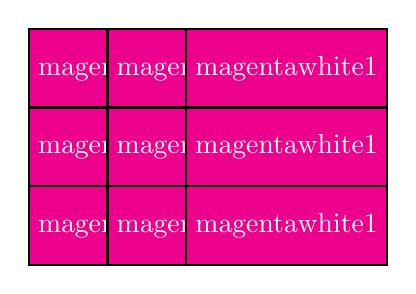
\begin{tikzpicture}
    \begin{scope}[thick,local bounding box=name]
    
         \ColorCells{
            1/1/magenta/1,
            2/1/magenta/1,
            3/1/magenta/1,
            1/2/magenta/1,
            2/2/magenta/1,
            3/2/magenta/1,
            1/3/magenta/1,
            2/3/magenta/1,
            3/3/magenta/1
         }

    \end{scope}
\end{tikzpicture}
} %%% case